\documentclass[a4paper,singleside,12pt]{report} % Uncomment this for single side pdf.
%\documentclass[a4paper,twoside,12pt]{report} % Uncomment this for printing.

\usepackage{ai_bo_thesis}
\usepackage[english]{babel}
\usepackage[T1]{fontenc}
\usepackage{lmodern}
\usepackage{amsmath}
\usepackage{amsfonts}
\usepackage{siunitx}

\usepackage[backend=biber,style=trad-plain, sorting=nty,firstinits=true]{biblatex}
\addbibresource{citations.bib}

\setmainfont{Times New Roman}
\begin{document}

        \title{Decentralized Coordination with Multi-Agent Reinforcement Learning and Communication among Agents}
        \topic{Autonomous and Adaptive Systems}
        \candidate{Giovanni Minelli}
        \supervisor{Prof. Mirco Musolesi}
%	\cosupervisor{& John Doe, PhD.} % One co-supervisor.
%	\cosupervisors{& Dott.~Ing.~Luigi Bianchi\\& Dott~Avv.~Lucia Rossi} % More than one co-supervisor.
	\academicyear{2021-2022}
	\session{7th}
	
	\frontispiece 
	\dedication{\small{\texttt{self.dedicatedTo(p) for p in Friends\&Family}}}
	\toc
	\figstoc
	\tablestoc
	\begintext

\thispagestyle{plain}
\begin{center}
    \Large
    \textbf{Abstract}
\end{center}

Coordination of actions plays a crucial role in multi-agent systems as it allows entities to work together towards a common goal or individually in a shared environment without hindering each other's progress. In order for this to occur, it is essential for them to be able to understand and acknowledge the respective intention. But achieving this level of spatial awareness and collaborative skill is a complex task, as real-world constraints such as limited knowledge acquisition, computation requirements, and communications with neighbouring agents must be taken into consideration. This thesis aims to contribute to the research field by studying coordination among agents habilitated to exchange information. The challenges and existing solutions are discussed, then an alternative view for solving the problem is presented. The paper argues that mechanisms to force coordination are unnecessary since agents that can freely choose whether to collaborate or not can be more proficient in general situations and still occasionally work together when it results in the best option. In support of this claim, CoMix, a novel architecture that reflects this strategy is proposed and evaluated on a large scale through thorough testing, showing beneficial results and strategic behaviours from agents in action.

\chapter{Introduction}\label{introduction}

Cooperation and competition are commonly studied behaviours in multi-agent environments, and state-of-the-art methods have shown great success in these tasks \cite{Silver2017MasteringCA, Zhang2020MultiAgentCV}, but, it is important to recognise that most real-world scenarios do not fit neatly into a defined category that includes one or the other. Instead, by focusing on coordination dynamics, it would be possible to develop methods enabling optimal system evolution regardless of individual objectives set by the environment \cite{Schrittwieser2019MasteringAG}. This will require tackling the difficult challenge of coordinated decision-making, but developments in this direction could lead to significant advances in technology applications, especially in areas involving social skills such as swarm robotics and timely interactions such as autonomous vehicle navigation.

\section{Multi-agent systems}\label{multi-agent-systems}

A Multi-agent System (MAS) encompasses multiple autonomous entities, referred to as agents, that interact with each other within a shared environment \cite{weiss1999multiagent}. The goal of each agent is to accomplish a specific task, and the behaviour required to do so can be quite complex, possibly requiring interactions of cooperative or competitive type, depending on the task at hand. Due to the complexity of such systems, instead of developing intelligent behaviours from scratch, it would be possible to inject intelligence into the agents, pre-programming responses to interactions, or adopting fixed shared rules which decrease the space of uncertainty. However, it is generally more desirable for agents to possess the ability to adapt and learn over time. One prominent framework for that learning ability is Reinforcement Learning (RL), which entails modifying behaviour through a process of trial and error.\\
Recent advances in Artificial Intelligence (AI) and Deep Learning (DL) have led to a surge of research interest in Multi-agent Reinforcement Learning (MARL). This approach has demonstrated success in a wide range of fields, including robotics, natural language processing, game playing, and network security. In particular, RL has been utilised to develop intelligent robots that can navigate and manipulate objects in their environment \cite{Albrecht2017AutonomousAM}; strategy selections for acting in impractical spaces explorations \cite{Silva2019ASO} or optimisation of resources \cite{Mnih2015HumanlevelCT}; in classic game playing it has been used to develop agents that can compete at human levels, such as playing chess, Go and poker \cite{Silver2016MasteringTG, Silver2017MasteringTG, Brown2018SuperhumanAF}, or in the case of strategic multiplayer online games where cooperation with other agents is required to achieve a common goal, such as DOTA 2 \cite{OpenAI_dota} and StarCraft II \cite{Vinyals2019GrandmasterLI}.\\
Despite the impressive results that can be achieved with deep reinforcement learning, its application to a multi-agent setting poses unique challenges: the concurrent and heterogeneous behaviour of the agents leads to an unpredictable environment, referred to as non-stationarity \cite{Shoham2007IfML, Buoniu2008ACS, HernandezLeal2017ASO}; the exponential explosion of states leads to the curse of dimensionality \cite{Shoham2007IfML, Buoniu2008ACS}, making it difficult to assign credit to specific agents for a given outcome \cite{Wolpert2001OptimalPF, Agogino2004UnifyingTA}; large action spaces coupled with the need for global exploration \cite{Matignon2012IndependentRL}, increasing the complexity of the learning process; the potential for relative overgeneralisation \cite{Fulda2007PredictingAP, Wei2016LenientLI, Palmer2017LenientMD}. For this reason, a successful single-agent RL methodology cannot be simply applied to a multi-agent setting without re-evaluating its learning approach.

\section{Coordination}\label{coordination}

Intelligent coordination refers to the coordinated effort of a group of agents who are able to make intelligent decisions to act not only on the basis of their own goals but taking into consideration other entities in the environment as well. It involves establishing a shared understanding of the task at hand and developing a plan that outlines the roles and responsibilities of each agent. This concept is a promising area of research in MARL as it addresses the challenges introduced by the presence of multiple entities, enabling more effective action selection and limiting inefficient behaviours.\\
In general, we seek coordination ability both in cooperative and competitive settings.

\begin{itemize}
    \item Cooperation refers to the act of working together towards a common goal. It involves the mutual support and assistance of multiple agents, each of whom contributes their own unique skills and abilities to the collective effort.
    \item Competition refers to the ability of agents to compete with each other to achieve their goals. It typically involves agents taking actions that maximise their own reward or utility, potentially at the expense of other agents.
\end{itemize}

Cooperative contexts are undoubtedly the most researched \cite{Cao2012AnOO} since their successful application among agents can lead to the achievement of greater goals beyond the capabilities of the single agent and the emergence of group intelligence. This is the foundation of many applications in robotics, swarm intelligence, and social studies. However, competition is also a vital aspect worth considering, as it can motivate agents to improve their performance and explore the environment more efficiently. Furthermore, competition can prevent agents from becoming too dependent on one another and encourage them to develop more sophisticated strategies. Despite this common distinction, it should be noted that usually, we do not have a clear cut between cooperative and competitive behaviour in most real-world scenarios. \cite{Buoniu2008ACS, Hoen2005AnOO} have pointed out that a cooperative agent may temporarily act selfishly while trying to achieve a common goal, and a competitive agent may temporarily form a coalition with its opponent to achieve its own goal. Therefore, when designing a coordination system, it is important to avoid injecting a fixed criterion for collaboration or obstruction.

\section{Information Sharing}\label{information-sharing}

Intelligent agents (whether humans or artificial) can greatly benefit from the ability of information exchange to coordinate, strategise, and combine reciprocally their sensory experiences to act in the environment. Indeed, it is usually assumed that agents placed in the real world have to operate in situations of partial observability, limited in their knowledge and perception of their surroundings, and it would be unrealistic to assume otherwise.\\
By enabling communication, we can aid the agent in gathering information about the environment and improve its decision-making process by sharing observations, action policies, future intentions, or other relevant information. Furthermore, communication enables agents to form strong relationships and work together in groups, leading to improved behaviours and increased efficiency in task completion. This is achieved through the parallelisation of activities and optimisation of resources where local neighbourhoods allow reductions in the number of messages exchanged and computations wasted. We can see examples of this ability in a wide range of RL applications, like multi-player gameplay in environments simulated (e.g., DoTA, StarCraft) or physical (e.g., robot soccer), and in real applications like self-driving car networks working together for safe and efficient transportation or teams of robots deployed in hostile and rapidly-evolving environments, as well as many others.

\section{Centralised decision}\label{centralised-decision}

When trying to achieve coordinated behaviour, a straightforward approach is to adopt a hierarchical structure, where one agent takes on the role of coordinator to establish order and take effective decisions for the system evolution. However, the question arises of who should be in charge of this role and who better understands the situation. Approaches based on centralised coordination delegate the responsibility of coordinating the agents to a single agreed-upon entity, but even if a reliable hierarchical mechanism is in place, the question remains: How can the higher-level agent acquire the necessary information and successfully coordinate all other agents? How can this method address scalability and generalisation to different situations?\\
An alternative and often preferred approach is a decentralised one, where there are no agents with higher roles controlling the behaviour of others. This method eliminates the difficulties associated with centralisation, such as global coordination and scalability issues. On the other hand, agents in a decentralised system have limited knowledge and must rely solely on their local information, which increases uncertainty and variability of action and makes it difficult to predict the overall behaviour of the group. As a result, this leads to suboptimal policies and ineffective interactions during testing, especially when complex coordination is required. In particular, the problem has been widely studied under the name of interactive consistency, or in a more restricted setting as Byzantine generals, where the agents have to take a group action with shared consensus to succeed.

\section{From Simulation to Reality}\label{into-the-real-world}

<In the field of RL research, there is often a strong desire to achieve realism and, when possible, to deploy agents in real-world settings. However, using black box algorithms such as deep neural networks, for decision-making, can make it difficult to transfer these agents from simulated environments to the real world in laboratory or production settings because of a lack of explainability and predictability and because of the gap between a training and testing environment>. To address this difficulty, there has been a trend towards using more realistic simulation environments and combining RL and robotic research efforts. Thanks also to independent organisations \cite{UnityML} and open source communities \cite{Farama}, many simulated environments are available to test physics interactions, structural properties, and complex behaviour at scale. <In this thesis, the aim is also to gain good insights into the proposed algorithm's performance in a more realistic environment>.

It is also worth mentioning that the communication process plays a key role in RL. There is a vast research activity in the telecommunication field and under the Internet of Things (IoT) umbrella, that tries to design infrastructure and cope with interconnected entities limited in their computation and decision ability. However, this thesis will not cover the physical aspects that agents deployed in real scenarios are usually subject to, such as unreachability or disrupted communications. The analysis and reasoning will assume an agent-to-agent (A2A) communication, following the traditional device-to-device (D2D) paradigm, where physically close devices (e.g., two agents), can communicate directly over a so-called sideline. Compared to regular centralised uplink-downlink communication, D2D communications benefit from a shorter link distance and fewer hops, which is better in terms of reliability. Moreover, since communication is direct, i.e., without intermediate nodes, D2D has the potential to provide lower latency in the transmission of information.

These topics represent central points of the research field, and developments in their directions are crucial for the extensive use of AI in the wild. The central focus of this thesis work is the development of new architectures and strategies for autonomous agents operating in shared environments. Specifically, the research aims to investigate the ability of agents to learn autonomously, to act, and purposely coordinate when necessary. The proposed architecture and strategies described in the following chapters aim to answer the following research questions:

\begin{itemize}
\item Can agents acting in a shared environment with the ability to communicate, learn autonomously when coordination is necessary and preferable to selfish behaviour?
\item Is it possible to design an action strategy for independent agents that uses simple communication to achieve effective group coordination?
\end{itemize}

The aim, therefore, is to demonstrate, under different constraints and needs, whether a consensus in behaviour can be reached through the individual striving for a better reward without forcing coordination.


\chapter{Background}\label{background}
This chapter provides a comprehensive introduction to reinforcement learning and multi-agent reinforcement learning. Beginning with a naturalistic explanation of the mechanisms involved, it proceeds by discussing the taxonomy of problems and tractability properties. The focus then shifts to the area of communication and coordination mechanisms, which constitutes the core of this dissertation project.

\section{Origins and Definition of Reinforcement Learning}\label{origins}

The field of RL has its origins in the study of animal learning and behaviour, specifically in the psychological literature \cite{Rao2000ReinforcementLA} and animal experimentation \cite{Rescorla1988behavioral}, which have shown that animals can learn to perform complex tasks through trial-and-error, with the help of rewards and punishments. Later, the concept of RL was formalised in the field of artificial intelligence, where it is defined as a type of learning in which an agent learns to perform actions that maximise a scalar reward signal. The agent's goal is to learn a policy, which is a mapping from states of the environment to actions, that maximises the expected cumulative reward over time \cite{Rao2000ReinforcementLA}.

The standard mathematical framework for modelling sequential decision-making problems is the Markov decision process (MDP), which is defined as a tuple \(M = (S, A, P, r, \gamma)\), where:

\begin{itemize}
\item
  \(S\) is the state-space, a finite set of world states, represented as \(S = {1, 2, \dots, |S|}\).
\item
  \(A\) is the action-space, a finite set of actions, represented as \(A = {1, 2, \dots, |A|}\).
\item
  \(P(s_{t+1}|s_t, a)\) is the state transition probability function that expresses the probability of transitioning from state \(s_t\) to state \(s_{t+1}\) by selecting action \(a\).
\item
  \(r = R(s_t, a, s_{t+1})\) is the reward obtained from the reward function, given the transition from state \(s_t\) to state \(s_{t+1}\) by taking action
  \(a\).
\item
  \(\gamma \in [0, 1]\) is the discount factor, which is used to handle both finite and infinite-horizon problems.
\end{itemize}

The goal of an RL agent in a MDP is to find a deterministic, optimal policy \(\pi^*: S \rightarrow A\), which will dictate how the agent should act in order to maximise its rewards. Mathematically, the optimal policy can be defined as,

\begin{equation}
\pi^* = \arg \max_{\pi \in \theta} \mathbb{E}[\sum_{t=0}^{\infty} \gamma^t R(s_t, \pi(s_t), s_{t+1}) \mid s_0 = s]
\end{equation}

where \(\theta\) is the set of all admissible deterministic policies, and \((s_0, a_0, s_1, a_1, \dots)\) is a state-action trajectory generated by the Markov chain under policy \(\pi\). The optimal policy is the one that maximises the expected cumulative reward over an infinite horizon.

An alternative to directly searching for the optimal policy is to define two utility functions that capture the concept of expected return. These are the value function and the state-action value function, also known as the Q-function. The value function for a given policy \(\pi\) is defined as:\\
${V^{\pi}(s) = E [\sum_{t=0}^{\infty} \gamma^tr(s_t, \pi(s_t))|s_0 = s]}$ \\
It encodes the expected cumulative reward when starting in state \(s\) and following the policy \(\pi\) thereafter.\\
The state-action value function, or Q-function, is defined as: 
${Q^{\pi}(s, a) = E [\sum_{t=0}^{\infty} \gamma^tr(s_t, \pi(s_t))|s_0 = s, a_0 = a]}$ \\
It measures the expected cumulative reward when starting from state \(s\), taking action \(a\), and then following the policy \(\pi\). In the context of deep reinforcement learning, the policy, the value functions, or both are typically represented by neural networks.

\section{MARL}\label{marl}

In multi-agent reinforcement learning, we extend the single-agent case
by introducing a different formulation known as a Markov Game. This is a
generalisation of Markov Decision Processes and allows for modelling
more complex decision-making scenarios where agents need to make
strategic decisions based on the actions of other agents. In a Markov
Game, each agent acts according to its own policy, which may differ from
one agent to another, affecting each other's rewards and future states.
This is formalized by the tuple \((N, S, {A_i}, P, {R_i}, \gamma)\),
where:

\begin{itemize}
\item
  \(N = \{1, \dots, n\}\) denotes the set of \(n > 1\) interacting agents
\item
  \(S\) is the set of states observed by all agents
\item
  \(A = A_1 \times \cdots \times A_n\) joint action space is the
  collection of individual action spaces from agents \(i \in N\)
\item
  \(P: S \times A \rightarrow P(S)\) is the transition probability
  function and describes the chance of a state transition
\item
  \(R_i\) is the reward function defined as
  \(R_i: S \times A \times S \rightarrow \mathbb{R}\) associated to each
  agent \(i \in N\)
\item
  \(\gamma \in [0,1]\) is the discount factor.
\end{itemize}

At stage \(t\), each agent \(i \in N\) selects and executes an action based on the individual policy \(\pi_i: S \rightarrow P(A_i)\). The system evolves from state \(\textbf{s} = \{s_1, \dots, s_n\}\) under the joint action \(\textbf{a}\) with respect to the transition probability function \(P\) to the next state \(\textbf{s}'\), while each agent receives \(\textbf{r}\) as immediate feedback to the state transition. The goal of each agent, similar to a single-agent problem, is to modify its policy in order to maximise its long-term rewards \cite{Rao2000ReinforcementLA}.

\section{Taxonomy of the problem}\label{taxonomy-of-the-problem}
% Coop/Coord/Mixed %
The study of MAS often involves categorising situations using standard taxonomies to understand the system's characteristics clearly, compare it with other multi-agent systems, and identify specific challenges and opportunities. For example, we can distinguish between settings where the rewards obtained are shared or individually assigned. The relative taxonomy classifies them as:

\begin{itemize}
\item \textbf{Fully cooperative} setting, in which all agents receive the same reward for state transitions, i.e. $R = R_i = \dots = R_N$. Agents are motivated to collaborate in order to maximise the performance of the team.
\item \textbf{Fully competitive} setting, where the problem is described as a zero-sum Markov Game. In this setting, the sum of rewards equals zero for any state transition, i.e. $R = \sum_{i=1}^N R_i(s, a, s') = 0$. Agents are motivated to maximise their own individual reward while minimising the reward of others.
\item \textbf{Mixed} setting, also known as a general-sum game, the setting is neither fully cooperative nor fully competitive, and therefore does not impose any restrictions on the goals of the agents.
\end{itemize}

% Centr/Decentr %
Another commonly used taxonomy regards the learning and execution process, where we have a distinction based on the information available to agents:

\begin{itemize}
\item
  \textbf{Decentralised} settings \cite{Bowling2002MultiagentLU, kapetanakis2002reinforcement}, are characterised by the presence of independent learners who are unaware of the existence of other agents and are unable to observe their rewards or actions. A lack of global observability and coordination among agents usually marks this type of setting.
\item
  \textbf{Centralised} settings \cite{hu2003nash, littman2001friend}, feature joint-action learners capable of observing the actions taken by all other agents a-posteriori. Usually, it is adopted to introduce coordination among agents and some level of global observability.
\end{itemize}

The rewards and information available to agents in MAS can significantly impact the complexity of the problem. In cases where all agents receive a common reward and have complete knowledge of the environment (fully observable and fully cooperative), the problem can be reduced to a single-agent problem, allowing for the identification of exact optimal policies without coordination among agents \cite{HernandezLeal2017ASO}. However, these assumptions are often not met in reality, and even if they were, it would be beneficial to factorise the joint stochastic policy into ${\pi(a \mid s) = \forall i\ \pi_i (a_i \mid s)}$ to avoid the exponential growth of the action space $A$ with the number of agents, which can make greedy action selection, exploration, and learning architectures intractable. On the other hand, this inevitably leads to the problem of partial observability, where agents must act and learn with limited knowledge of the state of the world. 

Another issue with independent agents is that it is akin to having N learning algorithms running in a simulated environment that is constantly changing due to unpredictable rules, as each agent is simultaneously learning a policy to interact with the environment. This effect of non-stationarity of the environment is referred to as the moving target problem and can be formulated as \(P(s' \mid s, a, \pi_1, \dots, \pi_N) \neq P(s' \mid s, a, \bar{\pi_1}, \dots, \bar{\pi_N})\), which is the change in transition probability function as a result of the co-evolution of all agents' policies.

As the focus of this thesis is on decentralised control settings under the assumption of partial observability, it is important to emphasise the difficulty of solving the decision problem for Decentralised Partially Observable Markov Decision Processes (Dec-POMDPs). In fact, computing even an approximately optimal policy for Dec-POMDPs is NEXP-complete \cite{Bernstein2000TheCO, Rabinovich2003TheCO}. Despite some recent empirical successes \cite{Leibo2017MultiagentRL, Foerster2016LearningTC}, finding an exact solution to Dec-POMDPs using Reinforcement Learning (RL) methods with theoretical guarantees is still an open research question. Nonetheless, by introducing the relaxation of free communication between agents, we can expand the knowledge of the agents and move the problem into P-SPACE \cite(Blondel2000ASO), without introducing unrealistic abstractions that can only be achieved in simulations.

\section{Communication and consensus necessities}\label{communication-and-consensus-necessities}
% Introduction of communication/consensus %
In order to achieve coordination among decentralised, independent agents, some form of communication and agreement on actions must be established. This can be thought of as a distributed optimisation problem, where consensus in policy development (the development of an optimal policy attainable in multi-agent contexts) is achieved through local computation and communication with neighbouring agents.

In standard consensus algorithms, we have a set of agents \(a_i\), from \(A={i \in 1, 2, \dots, N}\), each initialised with some initial value. To enable communication, we can imagine the agents being interconnected over a reliable communication network, ideally represented as an oriented graph. To reach consensus, every agent communicates with one another, exchanging values, locally processes the information, and then proposes a single value \(v_i\), drawn from the set \(S={i \in 1,2, \dots, M}\). The agents are said to reach a consensus if, from a certain time step \(t\), it holds, \(\lim_{t \to \infty} v_1^t = v_2^t = \dots = v_N^t, \quad \forall i \in V\) and for every set of initial values \(\in S^m\).

A consensus algorithm is considered to be formally correct \cite{Coulouris2012DistributedS} if it satisfies the following three conditions in every execution:

\begin{itemize}
\item \textbf{Termination}: eventually, all \texttt{correct} processes set their decision variable.
\item \textbf{Agreement}: the decision value of all \texttt{correct} processes is the same.
\item \textbf{Integrity}: if all \texttt{correct} processes propose the same value, then any \texttt{correct} process in the \texttt{decided} state must choose that value.
\end{itemize}

By keeping these conditions in mind but relaxing some strict constraints like the convergence to a single state value of consensus, this research will focus on the design of a method of agreement among agents to optimise the local policy for individual needs but in accordance with the group's intentions.

% byzantine generals %
% interactive consensus %

\section{Common Approaches}\label{common-approaches}
% MARL: common approaches %
MARL comprises all those approaches used to train multiple agents to learn to interact in a shared environment. Therefore, they are techniques designed to handle large environments, the added complexity of having multiple interacting entities and most often designed with scalability in mind \cite{Gronauer2021MultiagentDR, HernandezLeal2019ASA, Stone2022ASO}. One potential solution for addressing this challenge is to use imitation learning cite{ACM2018ImitationLearningSurvey}, in which agents learn to imitate the actions of an expert demonstrator by using a set of collected trajectories. For instance, \cite{Osinski2019SimulationBasedRL, Maramotti2022TacklingRA} uses this approach to transfer the driving ability of human experts to an agent that can control a physical car, reducing the need for extensive trial and error exploration of the enormous state space that characterises autonomous driving. However, this approach requires a significant amount of expert trajectories, which, being specific to the environment and task at hand, are hardly reusable for other tasks, as well as having the potential for overfitting during training.\\
Another relevant method is hierarchical reinforcement learning (HRL) \cite{MLKE2022HRLSurvey}. In HRL, the learning process is divided into multiple levels or layers of abstraction, with each one being used to represent the space or the goal with a different degree of granularity. For example, an RL agent learning to play a video game might have a lower level that focuses on actions such as moving and jumping, and a higher level that rewards strategies such as exploring the environment or attacking enemies. By breaking the learning process into multiple levels, HRL can simplify the problem and make it more manageable at scale. Indeed, it is currently considered a state-of-the-art technique in the field of robotic control problems \cite{Nachum2018DataEfficientHR}. The downside is that HRL can be difficult to implement, as it requires careful design of the hierarchical structure and abstraction at each level, with the associated risk of leading to sub-optimal solutions during training or lack of generalisation.\\
On the other hand, we find extensions of single agent algorithms or fully decentralised approaches that focus on learning directly from the interactions of multiple agents in the environment, allowing them to handle non-stationary and changing environments more effectively.

\subsection{Centralised and Decentralised Approaches}\label{cendecenctde}
% Centr, Decentr, CTDE %
When dealing with simple MARL applications, we can adopt a centralised approach where the environment is viewed as a whole and the interactions between agents are observed from a global perspective. While this simplifies interactions and makes policy computation easier, it would not be suitable for the scalability of the system, a requirement that has recently attracted much attention in the development of new methods \cite{Gronauer2021MultiagentDR, HernandezLeal2019ASA, Stone2022ASO}. Additionally, the assumptions of centralisation can be difficult to achieve in practice, as it may not reflect the reality of a scenario with a central entity in the system.\\
An alternative approach is decentralised control, where each agent makes its own decisions independently, without the need for a central controller or global coordination. The independent learning framework can obtain good empirical performance in several benchmarks \cite{Papoudakis2020BenchmarkingMD}, but there are few theoretical guarantees for decentralised learning, and the interpretability is often insufficient.
Recent work has focused on a hybrid approach \cite{Lowe2017MultiAgentAF, Foerster2017CounterfactualMP, AAMAS2018VDN, Rashid2018QMIXMV}, where global information is required only during the training phase, allowing the algorithm to be free of the need for continuous awareness of other agents' behaviour during the testing phase. Centralised Training with Decentralised Execution (CTDE) is one such approach, which has been expanded into two main lines of research that align with standard MARL frameworks. Actor-critic models, such as Multi-Agent Deep Deterministic Policy Gradient (MADDPG) \cite{Lowe2017MultiAgentAF}, use a centralised per-agent critic to estimate the Q-function and decentralised actors to optimise the agents' policies. There is no explicit communication in this approach, as the other agents' actions are inferred from their respective policies. Another similar approach is Counterfactual Multi-Agent (COMA) \cite{Foerster2017CounterfactualMP}, which addresses the challenges of multi-agent credit assignment by using a counterfactual baseline that marginalises out a single agent's action while keeping the other agents' actions fixed. However, these actor-critic models require on-policy learning, which can be sample-inefficient, especially when the state space is large.\\
An alternative CTDE approach is to learn a centralised Q-function \cite{AAMAS2018VDN, Rashid2018QMIXMV, Son2019QTRANLT, Yang2020QattenAG, Wang2020QPLEXDD}, in which the optimality is reached by considering the relationship between joint action value and optimal local actions. For example, Value Decomposition Networks (VDN) \cite{AAMAS2018VDN} learn the joint-action Q-values by factoring them as the sum of each agent's Q-value, and QMIX \cite{Rashid2018QMIXMV} extends VDN to allow the joint action Q-function to be a monotonic combination of each agent's Q-value that can vary depending on the global state. Despite achieving excellent results, QMIX has faced criticism for its limited representation capacity due to the monotonic constraint, and several alternatives have been developed to address this limitation. Between the most important, we find QTRAN \cite{Son2019QTRANLT}, which learns an unrestricted joint action-value function and aims to solve a constrained optimisation problem in order to decentralise it, and QPLEX \cite{Wang2020QPLEXDD}, which takes advantage of the dueling network architecture to factor the joint Q-function in a manner that does not restrict the representational capacity. In this thesis, I will use the advances of the centralised Q-function approach to teach agents functional behaviour in a non-stationary environment characterised by partial observability.

\subsection{Communication channel}\label{communication-channel}
% Communication channel %
Mechanisms for information sharing and communication are introduced to reduce non-stationarity effects \cite{Heider1944AnES, Rasouli2017AgreeingTC}. Communication between agents can take the form of explicit communication using talk channels, or implicit communication by observing other agents' actions or their effect on the environment. <>In the former case, one option is to rely on standardised message formats, such as the Agent Communication Language (ACL), to enable independent agents to communicate with a precisely defined syntax, semantics and pragmatics \cite{Poslad2007SpecifyingPF, Finin1994KQMLAA}. On the other hand, ad-hoc communication protocols with learnt communication are mostly adopted when complex coordination is required. Even though the first approach may result in a lack of generality and flexibility due to the imposed structure, having a standardised and well-defined structure is helpful when the goal necessitates common understanding. Some research tries to find a balance between standardisation and flexible communication taking the best of both approaches \cite{Luncean2015CommunicationAI, Koes2004CommunicationEI}.\\
Efficiency, as well, is a common driver in designing effective communication, as real-world environments involve other factors such as security overhead, message brokering time and dynamism of the whole environment. There are differing opinions on the best format to adopt for messages (structured, discrete, continuous, etc.) \cite{Lowe2017MultiAgentAF, Koes2004CommunicationEI, Li2021LearningED, Sukhbaatar2016LearningMC}, and the optimal method for exchanging information in terms of costs and benefits. Some methods include using a common memory buffer where agents can write and read to share information \cite{Pesce2019ImprovingCI}, adopting an event-based framework where communication occurs only under certain circumstances \cite{Hu2021EventTriggeredCN}, and integrating implicit communication by observing the actions of others and inferring their policies to reduce the communication needs \cite{Ding2020LearningII}.\\
Communication can take place in one or both directions: direct messages are shared between two agents by opening a communication channel \cite{Niu2021MultiAgentGC, Zhao2022TargetedMC}, or by broadcasting it to everyone \cite{Kim2021CommunicationIM, Lin2021LearningTG, Sukhbaatar2016LearningMC, Das2018TarMACTM}. The latter approach is more expressive under partial observability assumptions, but it is also more expensive in terms of transmission traffic and can lead to irrelevant information overwhelming the relevant information in crowded settings. Some approaches aim to create smaller groups of agents that focus on inter- and intra-correlation to limit irrelevant reasoning and improve coordination performance \cite{Liu2021LearningCF, Niu2021MultiAgentGC, Liu2020When2comMP, Niu2021MultiAgentGC, Jiang2018LearningAC}. Others reduce the number of messages sent by learning to understand when communication is really necessary or when the information held is redundant and communication avoidable \cite{Liu2020When2comMP, Ding2020LearningII}. Some solutions aim at targeting communication to those who are interested in it \cite{Zhao2022TargetedMC}, while others act on the side of the listener by adopting different mechanisms of attention to filter out irrelevant messages \cite{Li2021LearningED, Kim2021CommunicationIM, Sukhbaatar2016LearningMC, Das2018TarMACTM}. While these methods of obscuration or filtering are often effective, they typically do not take into consideration the messages in the context of the whole communication channel, but are filtered only for their relevance to the individual agent, ignoring possibilities of more complex coordination.\\
Lastly, the simplification of designing architectures that encourage cooperation has greatly facilitated research in this direction \cite{Foerster2017CounterfactualMP, Li2021LearningED, Liu2021LearningCF, Mao2017ACCNetAN, Ding2020LearningII, Sukhbaatar2016LearningMC}, in contrast to mixed environments \cite{Tu2021AdversarialAO, Blumenkamp2020TheEO} where the lack of a rigid assumption of cooperation to succeed can make the task more challenging. This work, in particular, does not impose a fixed structure on communication, while maintaining a focus on efficiency, and does not limit its applicability only to cooperative frameworks.

\subsection{Message content}\label{message-content}
% What, when communicate and how to include the info in your choices %
The message content is a crucial aspect for the recipient agent. It should be designed to provide additional information about the communicator's perspective, reducing uncertainty about their behaviour and facilitating coordination. One option is to use a highly expressive message encapsulating the agent's reasoning process. For instance, some works \cite{Sukhbaatar2016LearningMC, Singh2018LearningWT, Das2018TarMACTM, Peng2017MultiagentBN} have structured their architectures around recurrent modules, using the hidden state as a signal message for others. However, this is typically used internally to encode past and current information and reusing the individual reasoning vector for communication intent can have limiting effects in difficult tasks. Other works \cite{Sukhbaatar2016LearningMC, Singh2018LearningWT} merge multiple incoming messages into a single communication vector using weighted operations, which may not result in strong coordination when many agents participate in the communication.\\
\cite{Das2018TarMACTM, Jiang2018LearningAC} use crafted messages to transmit elaborate information to others and train successful agents able to understand each other. They also use weight sharing between agents, which is quite common \cite{Kim2021CommunicationIM, Das2018TarMACTM, Peng2017MultiagentBN, Jiang2018LearningAC} to reach a better action understanding and counteract scalability issues. Nevertheless, this implies that agents have the same reasoning ability on a piece of information, which may not be an accurate representation of the agents' individual abilities and affect the learning process of policies to be effective for the average agent, but not for each individual.\\
More straightforward transmission approaches \cite{Liu2020When2comMP, Kim2021CommunicationIM} use current or time-delayed observation as a communication message, usually with additional information expressing intentions. This implementation delegates most of the interpretation and coordination to the receiver but allows for more flexible interaction dynamics. In combination with the use of a module to learn a better representation \cite{Lin2021LearningTG}, this method can also be used without the burden of raw information exchange.\\
Finally, in some cases we can even ignore the content of the message and, assuming full mutual knowledge of each other, the effort will only be focused on learning a policy expressing coordination. Previous works \cite{Ren2005ConsensusSI, OlfatiSaber2007ConsensusAC} included the use of a mechanism where the consensus is mandatory in order to proceed, while current methods implemented with agents able to "learn", prefer a looser agreement, aiming instead to obtain convergence in target choice and coordination in actions. For example, \cite{Li2021StructuredDE} forms groups of agents with similar objectives to have tighter cooperation and diversity of action between teams, but the proposed architecture is not end-to-end differentiable.\\
The main point of this work is that coordination should not be considered as a general requirement, but rather only in certain situations, as extensive reasoning on others' beliefs and intentions can slow convergence to a good individual policy and even be harmful.

\chapter{Approach}\label{approach}

In this section, the proposed solution for addressing the issue of coordination in MAS will be presented. This project work utilises established algorithms and principles to make significant contributions in terms of the implementation of reasoning processes for MARL agents. The claims are supported in the next chapter by thorough testing in two different scenarios with a particular focus on scalability performance, and by conducting an ablation study to assess <the impact of each aspect of the architecture>.

\section{Description}\label{description}
% from critics to description %
The traditional approach to address the problem of coordination in MARL systems is to prioritise coordination over other individual considerations. While this approach may be appropriate in scenarios where cooperation is the only way to succeed, it can prove detrimental in scenarios where agents are permitted to exhibit different behaviours to achieve their own individual goals.\\
An intuitive example of this is a car driver who wants to go from a starting point to their destination. If the driver were to constantly consider the intentions and actions of other drivers at each "step" of the trip, evaluating the possibility of allowing another driver to go first or taking the lead themselves, the trip would become endless. This reasoning is accentuated in large and sparsely-rewarded environments, where it is harder to extract rules and the exponential possibilities of interactions with others can lead to high uncertainty of action and slow down the convergence to a good policy or suboptimal convergence.\\
Another critique of this approach is the reliance on complex communication channels for establishing coordination. The primary goal of communication should be to reduce uncertainty and non-stationarity effects by providing additional information about the actions and intentions of other agents. However, many methods rely on the exchange of complex vectors that encapsulate agents' history or personal thoughts, which can be cryptic for thirds. This can make it difficult for agents to fully understand the true intentions of the speaker in a general context. Additionally, complex environments are more challenging in terms of state evaluation, thus it is important to keep the size of the state space small by providing agents with only relevant information.\\
As a final thought, the proposed work does not claim a declarative and imperative agreement between agents since coordination can arise from continued interactions. In fact, since all agents are subject to the same environmental rules, they will eventually avoid self-damaging decisions and occasionally cooperate to maximise their respective reward signals.\\
On top of that, I propose a policy that can adopt both egoistic and altruistic behaviours, a reasoning process that takes into account information from other agents, and a simple yet effective communication channel for exchanging information. The architecture of coordination and policy modules is implemented with recurrent neural networks to maintain consistency in decisions over time and is trained using a centralised training decentralised execution paradigm. Details of each module are discussed in the following sections, and the overall architecture is depicted in figure \ref{fig:pipeline}.


\begin{figure*}
  \centering
  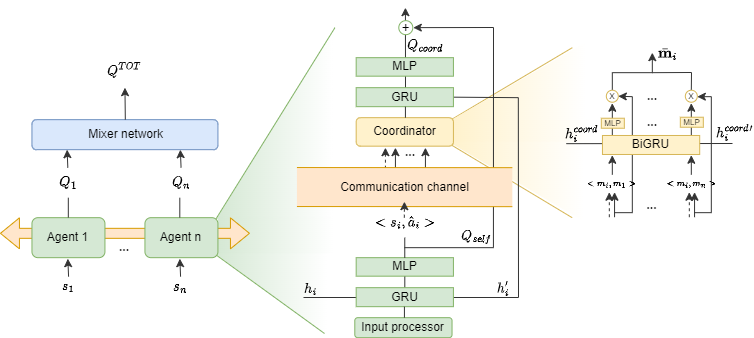
\includegraphics[height=5cm]{images/pipeline.png}
  
  \caption{ \textbf{CoMix architecture.} The figure depicts the CoMix architecture, with each module expanded into its components from left to right. (a) Individual agents are trained under a CTDE framework, with a mixer network used only during training that takes partial observations and state-action values to evaluate the system's performance. (b) At each step, the agents partially observe the environment and process the information to produce an independent choice of action, $Q_{self}$, which is then communicated through a communication channel. Every agent then considers all received messages to decide how to modify its previous selfish decision, producing the additional term $Q_{coord}$, which incorporates additional information filtered by the Coordinator. (c) The Coordinator computes a boolean mask to filter the communication channel, taking into account each neighbouring agent's communicated intention in relation to personal objectives. All decision-making components are implemented with recurrent modules to maintain consistency over time and enable agents to develop more structured strategies.}
  \label{fig:pipeline}
\end{figure*}\

\subsection{Action policy}\label{action-policy}

The Q network is responsible for predicting the state-action value for each action of an agent based on the information at his disposal. We can define it with the following formula: $Q_i(s_i,a_i,h_i)$ where $s_i$, $a_i$, and $h_i$ are the observation, action and hidden state of agent $i$ respectively. This would be considered sufficient for an implementation of an independent learner, however, in this setting, we incorporate communication messages as additional information that can aid the decision-making process when available. To achieve this, we reformulate the previous definition as the sum of two terms: $Q_i = Q_{self} + Q_{coord}$. Here, $Q_{self}$ represent the selfish action intention, which, once computed, produces state-action values for the current state and updates the hidden state for the next state $h_i \rightarrow h_i'$. The second term $Q_{coord}$ takes the current updated hidden state and incoming messages filtered out by a coordination module. Furthermore, the introduction of a feature extractor is made in the proposed solution. When executed on raw observation data, it extracts meaningful information, enabling the policy network to reason within a more defined space. It is worth noting that the input processing module used has shared weights among all agents. As highlighted by \cite{Lin2021LearningTG}, this is an important implementation detail to allow all agents to reason about data extracted from the same distribution.

The final formula representing the policy network involved is the following (subscript to indicate the timestep is omitted for brevity):

  \begin{equation}
    Q_i(s_i,a_i,h_i,\bar{\textbf{m}}_i) = Q_{self}(s_i,a_i,h_i) + Q_{coord}(a_i,h_i',\bar{\textbf{m}}_i)
  \end{equation}
  
The overall network is implemented with two GRU modules and linear layers to extract the value corresponding to each action for current agent's state $s_i$, sharing only the sequential hidden state vector. The recurrence of the first is necessary to process the new observation in relation to the past, while the second has the aim of properly mixing the self-interests with the new information obtained from other agents.


\subsection{Coordinator}\label{coordinator}

The coordination module is responsible for determining the relevance of other agents' communications in relation to the agent's intentions by producing a coordination mask used to filter out incoming messages. A message is defined as the communicated intention of an agent to take a certain action in order to achieve a personal objective, $\hat{a}_i=\arg\max_{a}Q_{self}(s_i,a,h_i)$, and is represented by the tuple \(m_i=<s_i,\hat{a}_i>\). Consequently, we define \(\textbf{m}\) as the set of incoming messages sent by \(n\) agents at a certain timestep \(\textbf{m}=\{m_1,\dots,m_n\}\) and \(\bar{\textbf{m}}_i\) as the filtered set for agent \(i\) obtained with the application of the communication mask \(\textbf{c}_i\), result of the Coordinator execution:

  \begin{equation}
    \textbf{z}_i=\{<m_i,m_1>, \dots ,<m_i,m_n>\}^{-<m_i,m_i>}
  \end{equation}
  \begin{equation}
    Coord(\textbf{z}_i)=\textbf{c}_i
  \end{equation}
  $ \text{ where } \textbf{c}_i=\{c_{i,1},\dots,c_{i,n}\}^{-c_{i,i}}$
  $\text{ and } c_{i,j}= 
    \begin{cases}
        1 & \text{if agent } i \text{ coordinate with agent } j,\\
        0 & \text{otherwise}
    \end{cases}$
  \begin{equation}
    \bar{\textbf{m}}_i=\textbf{m} \odot \textbf{c}_i
  \end{equation}
As previously proposed in \cite{Jiang2018LearningAC}, the module for this reasoning is implemented using a BiGRU layer, in order to take into account the intentions of all other agents under the same circumstances, but also in a reciprocal relation, \(\textbf{z}_i\). The individual scores produced by this layer are then used to calculate an independent probability of communication through a two-way softmax.

\subsection{Centralised network}\label{centralised-network}
Learning communication and action policy at the same time, in a setting of partial observability, may lead agents to inaccurately estimate their local Q function. The adoption of a CTDE learning algorithm prevents this, providing current state-action values $\textbf{q}$ and observations $\textbf{s}$ of the agents to a centralised network to learn a joint action-value function. The specific implementation used is the one proposed by \cite{Rashid2018QMIXMV}, which decomposes the joint function into factors depending only on individual agents, enabling it to cope with large joint action spaces. Therefore, when defining \(Q^{TOT}(\textbf{s}, \textbf{q})\), we have to respect the following two properties:

\begin{itemize}
\item
  \(Q^{TOT}\) yields the same result as a set of individual argmax operations performed on each \(Q_i\):
  \begin{equation}
  \arg\max_{\textbf{a}} Q^{TOT}(\textbf{s},\ulcorner\textbf{a},\textbf{h},\bar{\textbf{m}}\lrcorner) = \begin{Bmatrix}
  \arg\max_{a_1} Q_1(s_1,a_1,h_1,\bar{\textbf{m}}_1) \\
  \vdots\\
  \arg\max_{a_n} Q_n(s_n,a_n,h_n,\bar{\textbf{m}}_n) \\
  \end{Bmatrix}
  \end{equation}
\item
  The relationship between \(Q^{TOT}\) and each \(Q_i\) is constrained to be monotonic:
  \begin{equation}
  \frac{\partial Q^{TOT}}{\partial Q_i} \geq 0, \forall i \in [i,n]
  \end{equation}
\end{itemize}

Despite its limitations in terms of representational ability due to the monotonicity constraint, which limits QMIX to suboptimal value approximations, this algorithm has long been considered a state-of-the-art approach in the field. Nonetheless, the method proposed is not bound to the use of QMIX and can be adapted to different CTDE algorithms.

\section{Training}\label{training}

\subsection{Loss functions}\label{loss}
The agents' Q policy network is trained end-to-end with the error propagation being able to flow between the two reasoning processes by means of the hidden state shared. The rule of update for their parameters \(\theta^Q\) follows the common implementation of QMIX \cite{Rashid2018QMIXMV}, with the computation of a temporal difference error:
  \begin{equation}
    L(\theta^Q) = |y^{TOT} - Q^{TOT}(\textbf{s}, \textbf{q}; \theta^Q)|,
  \end{equation}
where $y^{TOT} = \textbf{r} + \gamma \max\limits_{\textbf{q}'}Q^{TOT}(\textbf{s}', \textbf{q}'; \theta^{Q}{'})$ and \(\theta^Q\), \(\theta^{Q}{'}\) are respectively the parameters of the online policy network and target policy network periodically copied from \(\theta^Q\) as in standard DDQN \cite{Van2016deep}. Note that compared to an individual network per agent, having a centralised function leads to considerably lower variance in policy gradient estimates since it takes into account actions from all agents. At test time, this is not needed, and policy execution is fully decentralised.

In designing an efficient learning schema for the coordination module, different options were evaluated following the same general intuition (TODO need testing time to understand if it is worth putting that in the ablation). Since the probability of communication produced by the single agent for each other sees its effects in a modified set of values for the state-action pairs, we can effectively measure it in an improvement or decrease in action performance by assuming an optimal estimate of the state-action value from the policy. Therefore, we can define the formula of update of the Coordinator's parameters as a clipped delta between the maximum state-action value obtained with filtered messages \(\bar{\textbf{m}}_i\) from the predicted mask of coordination with respect to the alternative estimated value obtained from messages filtered with inverted probabilities of communication
\(\tilde{\textbf{m}}_i = \textbf{m} \odot (1- Coord(\textbf{r}_i; \theta^C))\).
  \begin{equation}
    L(\theta^C)= \sum^n_{i=1} w_i \Delta Q_i = \sum^n_{i=1} w_i \max(0,\max_{a_i}Q_i(s_i,h_i,\tilde{\textbf{m}}_i,a_i) - \max_{a_i}Q_i(s_i,h_i,\bar{\textbf{m}}_i,a_i))
  \end{equation}

Following this reasoning, we can further improve the method at the cost of additional computation by performing $n-1$ inferences of the Q function, each considering a set of different messages. Instead of computing the Q value considering communicating with the opposite set of agents -- with respect to the predicted one -- we can compute an averaged expectation of the state action value, taking into account the advantage of reversing the communication probability per each single agent. Although this training implementation is much more expensive, it allows for improved results, especially when many agents are present. The choice is discussed further in the section dedicated to the ablation study (See \ref{ablation}).

The adoption of the QMIX approach gives us an additional element that can be used to better estimate the gain in using a mask of coordination in place of another. Being the mixer network a mapping from states to a set of weights in the hidden space used independently in linear combination with the action-state value of the respective agent, we can reuse these parameters to weight each \(\Delta Q_i\). In these terms, we can make updates more precisely related to the gain given by the communication with a certain agent in a certain state. We find mention of this in the above formula with the term \(w_i\).

\subsection{Training details}\label{training-details}
The training of the model incorporated randomness to capture the uncertainty of the predictions and to further explore the action space. On the coordinator side, coordination mask selection involved applying Gumbel Softmax to the two decision logits, which differs from the Softmax function by adding random noise from the Gumbel distribution to the output. For exploration in action selection, an epsilon decay technique was used, with the value decreasing from 0.9 to 0.05 over 60% of the training time.\\
To mitigate the risk of catastrophic forgetting and overfitting, a weight decay with a value of $0.0001$ was used as a regularisation term, and a soft update technique was adopted for the weights of the target network. The network sizes, learning rates and decay parameters were carefully chosen for each environment to optimise the algorithm's performance and achieve the best possible results. The learning algorithm was also found to be very sensitive to the number of recurrent steps considered during training, the value of which had to be chosen according to the task dynamics of each environment.

\chapter{Experiments}\label{Evaluation}
The aim of this chapter is to evaluate the proposed approach and its effectiveness in addressing the research questions stated earlier. The evaluation process will include a comparative analysis with other relevant methodologies in the field, followed by a presentation of the results obtained through a comprehensive and systematic evaluation process. The results will be examined in detail, including an examination of the proposed components and the implementation details, in order to identify overall strengths and limitations. In summary, this evaluation aims to shed light on the performance of the proposed methodology and enable the researcher to draw informed and insightful conclusions on its effectiveness in practical applications.

\section{Baselines of comparison}\label{Baselines}
\textbf{Individualised Controlled Continuous Communication Model} (IC3Net)\cite{Singh2018LearningWT} is proposed as an extension of a previous method \cite{Sukhbaatar2016LearningMC}, introducing a gating mechanism on each other agent's communication channel. They use the current observation encoded, both as internal thought and communication message, and a mask of communication to filter out incoming messages computed at the previous step. The reasoning process then occurs by processing the individual thoughts in an LSTM module and averaging the remaining incoming messages. The result is used as input to two output heads to obtain the action values and the individualised probability of communication.

\textbf{ATOC}\cite{Jiang2018LearningAC} is an attentional communication model proposed to learn effective and efficient communication at scale by adopting weight sharing between each agent's network. In their proposal, the communication message is represented by the hidden state of a recurrent module that processes the observation at each step, thus sharing a vector which resembles the agent's history. Based on the internal reasoning, the agent will decide whether or not to communicate with its neighbours, observing that this decision will create a group of maximum $m$ agents maintained for $T$ steps, with $m$ and $T$ as hyperparameters. The incoming messages from each group are mixed with a bidirectional LSTM module, where the final output is merged with the internal thoughts and processed to obtain the action values.
 
\section{Environments}\label{Environments}
For the evaluation, two testing environments were considered. The first of these is the \textbf{Switch} environment (Fig. \ref{fig:switch}), a grid world where four agents must navigate to reach their respective switch on the map, having as input only the current position and target distance. The agents are faced with a challenge due to the map's layout, which features two rooms with starting points and a narrow hallway connecting them. However, the corridor can only be crossed by one agent at a time, meaning that coordinated behaviour is necessary to prevent the agents from getting stuck. It is worth mentioning that the agents are unable to see each other, and must therefore use a communication channel to gather information about the positions and intentions of their peers. The task ends after 250 steps of execution, or when all agents have successfully reached their destinations. 

\begin{figure}
  \centering
  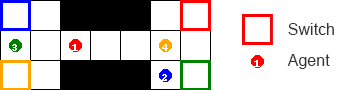
\includegraphics[height=2cm]{images/switch.png}
  \caption{\textbf{Switch Environment.} Four agents, with limited observation abilities, are tasked with reaching the switch of the corresponding colour. Coordination between the agents is necessary to avoid getting stuck in the corridor indefinitely.}
  \label{fig:switch}
\end{figure}

The second testing environment (Fig. \ref{fig:pursuit}) is an instance of the \textbf{Predator-Prey} problem provided by the PettingZoo library, which implementation requires particularly high levels of coordination to succeed. The environment consists of a grid world in which some agents chase randomly moving entities with the aim of capturing them. The pursuers have limited visibility of the world, extending up to three units in each direction from their positions, and same speed as the evaders. While an individual agent can only earn a small reward for "tagging" an evader (i.e., being in its same position), a group of organised agents can receive a larger shared reward "capturing" it (i.e., surround its position in the 4 axis). The task is considered complete either when all evaders have been captured or after 500 steps of execution.

\begin{figure}
  \centering
  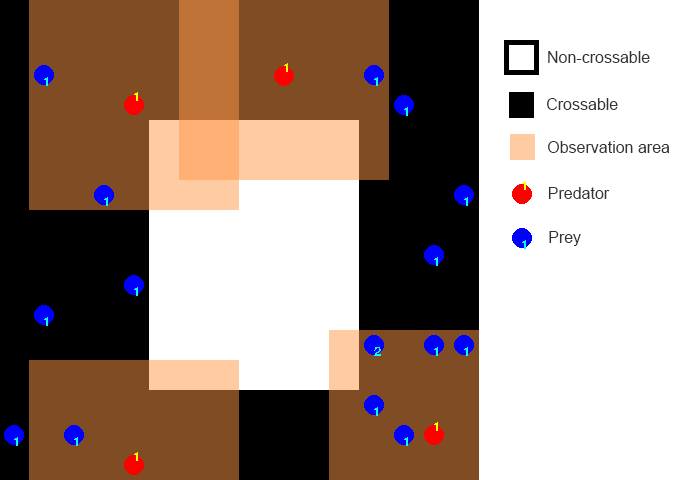
\includegraphics[height=9cm]{images/pursuit.png}
  \caption{\textbf{Predator-Prey Environment.} Pursuer agents navigate through space to capture prey. The agents' observation is restricted to a small area in their proximity, but they can communicate with other agents to gather additional information and coordinate their actions strategically.}
  \label{fig:pursuit}
\end{figure}


\section{Results}\label{results}
In evaluating the efficacy of the proposed method in comparison to the baselines, it is crucial to account for the disparity in the training methodologies employed. Specifically, IC3Net utilizes an on-policy training approach, in contrast to CoMix and ATOC. Furthermore, the latter two are trained with epsilon decay action selection, which allows for a more thorough exploration of the action space, but also leads to greater variance in the interactions with the environment.

\textbf{Switch} Figure X displays the learning curve of the CoMix method and the two baseline approaches in terms of the total reward received by the agents in an episode. A higher value indicates not only the agents' capability to reach their respective targets, but also their ability to do so in a minimal number of steps, since the reward decays from 10 to 5 during the agents' lifespan.
Given the simplicity of the task and its low potential for misunderstandings between agents, IC3Net's straightforward communication mechanism proves to be the most effective among the three methods compared. After about one thousand updates, the agents have already learnt almost deterministic behaviour and consistently obtain optimal rewards. CoMix follows, with slightly lower results, while ATOC struggles with the task. A deeper analysis of the latter reveals that in the execution, all agents tend to adopt the same action selection policy, moving in the same room. This usually ensures that at least two agents reach their intended target, while the others rarely show any further intention of turning back in the right direction. The behaviour is likely caused by weight sharing used for all components, which was not even mitigated by the introduction of an ID in the policy computation. On the other hand, IC3Net reaches optimal performance, likely because the task resolution requires low variability and therefore does not necessitate strong communication skills. If the task becomes too easy, the policy can adopt a deterministic action sequence, and the communication channel can become secondary. The CoMix method of communication and coordination maintains variability in the choices, which often leads to slower resolution but still enables all agents to reach their targets with high scores.

\textbf{Predator-Prey} 





\section{Ablation study}\label{ablation}





	\appendix
	
	\printbibliography[heading=bibintoc] % biblatex
	
	\acknowledgements
	   I'm very grateful to the inventor of the Lorem Ispum, without whom this thesis couldn't exist. I'd also like to acknowledge that without dolor I would not have been able to sit amet. Thanks a lot for that.
		
\end{document}